\documentclass[12pt]{article}
\usepackage[utf8]{inputenc}
\usepackage[margin=0.9in]{geometry}
\usepackage{paralist}
\usepackage{blindtext}
\usepackage{hyperref}
\usepackage{chngcntr}
\usepackage{amsfonts,latexsym,amsthm,amssymb,amsmath,amscd,euscript}
\usepackage{enumitem}
\usepackage{caption}
\usepackage{algorithm}
\usepackage{algpseudocode}
\usepackage{amsmath}
\usepackage[table,xcdraw]{xcolor}
\usepackage{tikz}
\usepackage{parskip}
\usepackage{fancyhdr}


    \hypersetup{colorlinks=true,citecolor=blue,urlcolor =black,linkbordercolor={1 0 0}}

\usetikzlibrary{calc}

\renewcommand\thesubsubsection{\arabic{subsubsection}}

\newenvironment{statement}{\color[rgb]{1.00,0.00,0.50} {}}{}


\newcolumntype{M}[1]{>{\centering\arraybackslash}m{#1}}
\newcolumntype{N}{@{}m{0pt}@{}}
\algnewcommand{\algorithmicand}{\textbf{ and }}


\algnewcommand\algorithmicforeach{\textbf{for each}}
\algdef{S}[FOR]{ForEach}[1]{\algorithmicforeach\ #1\ \algorithmicdo}


\newlist{enums}{enumerate}{3}

\setlist[enums, 1]{label={(\arabic*)}, noitemsep}
\setlist[enums, 2]{label={-}, noitemsep}

\hypersetup{
    colorlinks=true,
    linkcolor=blue,
    filecolor=magenta,      
    urlcolor=black
    }

\title{ADA Assignment 3}
% \author{Anirudh S. Kumar (2021517), Aakarsh Jain (2021507)}
\author{
    \\\vspace{0em} Anirudh S. Kumar \\\vspace{-0.5em}
    \footnotesize{Roll Number - 2021517}\\\vspace{-0.5em}
    \footnotesize{IIIT - Delhi}\\\vspace{-0.5em}
    \footnotesize{\href{mailto:anirudh21517@iiitd.ac.in}{\texttt{anirudh21517@iiitd.ac.in}}}
  \and
    \\\vspace{0em} Vartika\\\vspace{-0.5em}
    \footnotesize{Roll Number - 2021571}\\\vspace{-0.5em}
    \footnotesize{IIIT - Delhi}\\\vspace{-0.5em}
    \footnotesize{\href{mailto:vartika21571@iiitd.ac.in}{\texttt{vartika21571@iiitd.ac.in}}} 
    \vspace{1em}
}

\renewcommand{\footrulewidth}{0.4pt}% Default \footrulewidth is 0pt
\renewcommand{\headrulewidth}{0pt}% Default \headrulewidth is 0.4pt


\date{\today}

\begin{document}
\maketitle

\pagestyle{fancy}
\fancyhf{}
\fancyfoot[L]{Anirudh S. Kumar}
\fancyfoot[C]{\thepage}
\fancyfoot[R]{Vartika}

\section{Island of Sunland}
\subsection{Problem}

\begin{statement}
    The towns and villages of the Island of Sunland are connected by an extensive rail
network. Doweltown is the capital of Sunland. Due to a deadly contagious disease, recently, few
casualties have been reported in the village of Tinkmoth. To prevent the disease from spreading
to Doweltown, the Ministry of Railway of the Sunland wants to completely cut down the rail
communication between Tinkmoth and Doweltown. For this, they wanted to put traffic blocks
between pairs of rail stations that are directly connected by railway track. It means if there are two
stations x and y that are directly connected by railway line, then there is no station in between x
and y in that particular line. If a traffic block is put in the track directly connecting x and y, then
no train can move from x to y. To minimize expense (and public notice), the authority wants to
put as few traffic blocks as possible. Note that traffic blocks cannot be put in a station. It has to
be put in a rail-track that directly connects two stations.

Formulate the above as a flow-network problem and design a polynomial-time algorithm to solve
it. Give a precise justification of the running time of your algorithm.
\end{statement}

\subsection{Formulation as a Graph problem}
We can create a flow network where each node represents a station, and each edge represents a railway track connecting two stations. The source and sink in the network are Tinkmoth and Doweltown, respectively, with each edge's capacity being 1, as shown in Figure \ref{fig:network_flow}

\begin{figure}[ht]
\centering
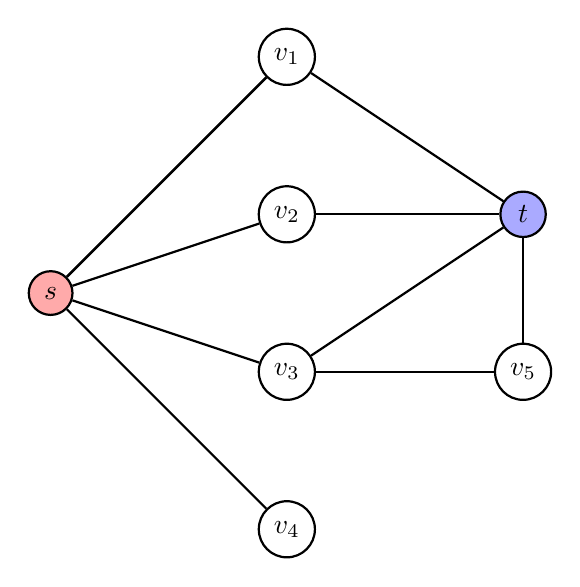
\begin{tikzpicture}[node distance={10mm}, thick, main/.style = {draw, circle}] 
	\node [main] (2) at (0, 3) {$v_1$};
        \node [main] (1) at (0, 1) {$v_2$};
	\node [main] (0) at (0, -1) {$v_3$};
        \node [main] (3) at (0, -3) {$v_4$};
	\node [main] (6) at (3, -1) {$v_5$};
	\node [main, fill={rgb:blue,1;white,2}] (5) at (3, 1) {$t$};
	\node [main, fill={rgb:red,1;white,2}] (7) at (-3, 0) {$s$};

    
    \draw[] (7) --  (1);
    \draw[] (7) --  (0);
    \draw[] (7) --  (3);
    \draw[] (7) --  (2);
    \draw[] (7) --  (2);
    \draw[] (2) --  (5);
    \draw[] (1) --  (5);
    \draw[] (0) --  (6);
    \draw[] (0) --  (6);
    \draw[] (0) --  (5);
    \draw[] (6) --  (5);



\end{tikzpicture}

\caption{An Example Network Flow Graph. Let each edge have weight 1. The source vertex is coloured red, and the sink is coloured blue.}
\label{fig:network_flow}
\end{figure}


\subsection{Algorithm for solving the problem}
To prevent the disease from spreading, we want to find the minimum number of traffic blocks required to cut off all paths from Tinkmoth to Doweltown.

Therefore we need to find the minimum cut in the network that separates Tinkmoth from Doweltown.

The minimum cut in the network that separates Tinkmoth from Doweltown will have a capacity equal to the minimum number of traffic blocks required to cut off Tinkmoth from Doweltown.
This is by the {\textbf{max-flow min-cut theorem}}.

 The {\textbf{maximum flow value}} in the network is equivalent to the minimum number of traffic blocks required to cut off Tinkmoth from Doweltown. This is because the flow from $S$ to $T$ represents the number of paths that can be established from Tinkmoth to Doweltown.

 Therefore, we can use {\textbf{Ford-Fulkerson Algorithm}} to find the maximum flow value.

\textbf{Remark:} The algorithm can also be used if the edge weights are not all 1 and there is an unequal flow between stations. 


 \subsection{Time complexity}

Ford-Fulkerson algorithm has a worst-case running time of $\mathcal{O}(f*|E|)$, where $f$ is the maximum flow, and $E$ is the number of edges in the network.
 In our case, $E$ will be the number of railway tracks connecting all stations. 
 
 Therefore the overall time complexity of our solution is $\mathcal{O}(f*|E|)$



\end{document}